\documentclass[a4paper,titlepage]{article}
\usepackage[utf8]{inputenc}
\usepackage{fullpage}
\usepackage{amssymb}
\usepackage{indentfirst}
\usepackage[per-mode=symbol]{siunitx}
\usepackage{listings}
\usepackage{graphicx}
\usepackage{color}
\usepackage{amsmath}
\usepackage{mathtools}
\usepackage{array}
\usepackage[hidelinks]{hyperref}
\usepackage[format=plain,font=it]{caption}
\usepackage{subcaption}
\usepackage{standalone}
\usepackage[nottoc]{tocbibind}
\usepackage[noabbrev,capitalize,nameinlink]{cleveref}
\usepackage{listings}
\usepackage{xspace}
\usepackage{tikz}
\usepackage{circuitikz}
\usepackage{titlesec}
\usepackage[cache=false]{minted}
\usepackage{booktabs}
\usepackage{csvsimple}
\newcommand{\MATLAB}{\textsc{Matlab}\xspace}
\usepackage{siunitx}
\usepackage[super]{nth}
\usepackage[titletoc]{appendix}

% Custom commands
\newcommand\numberthis{\addtocounter{equation}{1}\tag{\theequation}}
\newcommand{\code}[1]{\texttt{#1}}
\newcolumntype{P}[1]{>{\centering\arraybackslash}p{#1}}

\tikzstyle{my help lines}=[gray,thick,dashed]

\setminted{linenos,breaklines,fontsize=auto}

%\titleformat*{\section}{\normalsize\bfseries}
%\titleformat*{\subsection}{\small\bfseries}
\renewcommand{\thesubsection}{\thesection.\alph{subsection}}
\providecommand*{\listingautorefname}{Listing}
\newcommand*{\Appendixautorefname}{Appendix}

%opening
\title{\textbf{ECSE 543: Numerical Methods} \\ Assignment 3 Report}
\author{Wenjie Wei \\ 260685967}
\date{\today}

\begin{document}
	\sloppy
	\maketitle
	
	\tableofcontents
	\newpage
	
	\twocolumn
	\section*{Introduction}
		This assignment explored the use of linear interpolations and other mathematical methods. The programs are programmed and compiled using Python 3.6, and the plots are generated using package matlibplot. Listing \ref{lst:poly} shows the implementations of polynomials including their possible maneuvers. The object classes included in this file will be used for the interpolations. 
		
	\section{Linear Interpolation of BH Points}
		\subsection{Lagrange Full Domain Interpolation of First Six-Point Set}
			Listing \ref{lst:interp} shows the implementation of various interpolation methods. For the first six points, the Lagrange interpolation shows an interpolated polynomial
			\begin{align*}
				B(h) = &9.275\times 10^{-12}h^5 - 5.951\times 10^{-9}h^4 \\
					   &+ 1.469\times 10^{-6}h^3 - 1.849\times 10^{-4}h^2 \\
					   &+ 1.603\times 10^{-2}h
			\end{align*}
			whose plot is shown in Figure \ref{bh_first6}. 
			\begin{figure}[!h]
				\centering
				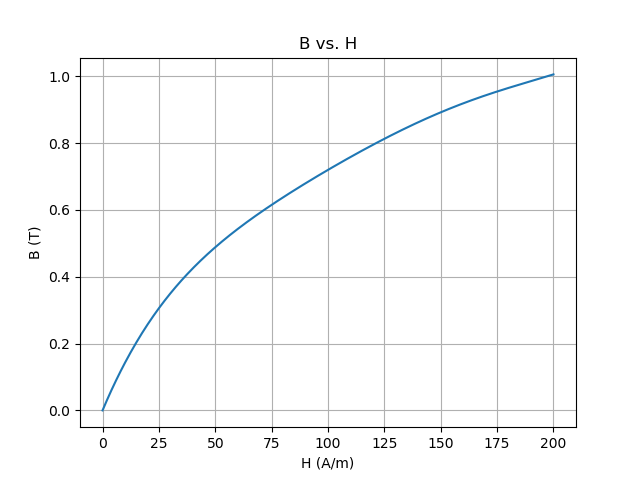
\includegraphics[width=\linewidth]{../data/B_H_first_six}
				\caption{Interpolation of the First Six Data Points}
				\label{bh_first6}
			\end{figure}
		
			From the figure, the interpolation has returned a plot with a \textbf{plausible} result over this range. 
		\subsection{Lagrange Full Domain Interpolation of the Second Six-Point Set}
			Select a second data point set, the Lagrange interpolation returned a polynomial of 
			\begin{align*}
				B(h) = &7.467\times 10^{-19}h^5 - 3.505\times 10^{-14}h^4 \\
					   &+ 5.3\times 10^{-10}h^3 - 2.864\times 10^{-6}h^2 \\
					   &+ 3.804\times 10^{-3}h
			\end{align*}
			whose plot is shown in Figure \ref{bh_second6}. 
			\begin{figure}[!h]
				\centering
				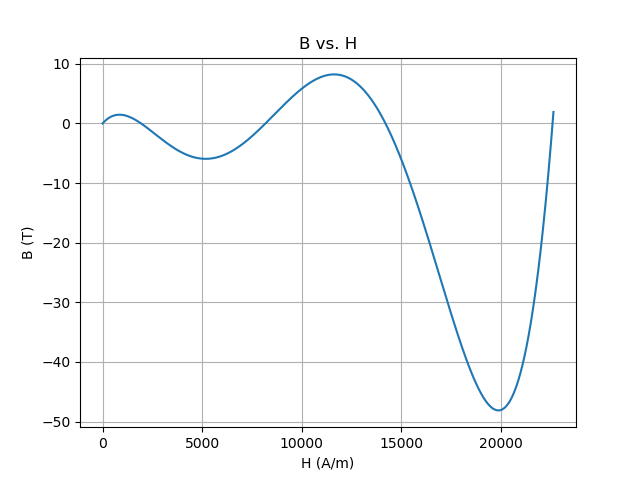
\includegraphics[width=\linewidth]{../data/B_H_second_six}
				\caption{Interpolation of the Second Six Data Points}
				\label{bh_second6}
			\end{figure}
			
			From this plot, we can see that the interpolation using the second set of data points is \textbf{not plausible} as the graph fluctuates violently as the value of $B$ goes to negative at some ranges. 		
		
		\subsection{Cubit Hermite Polynomial Interpolation}
			
		\subsection{Nonlinear Equation of the Magnetic Circuit}
			Consider the magnetic circuit shown in Figure \ref{mag_circuit}. 
			\begin{figure}[!h]
				\centering
				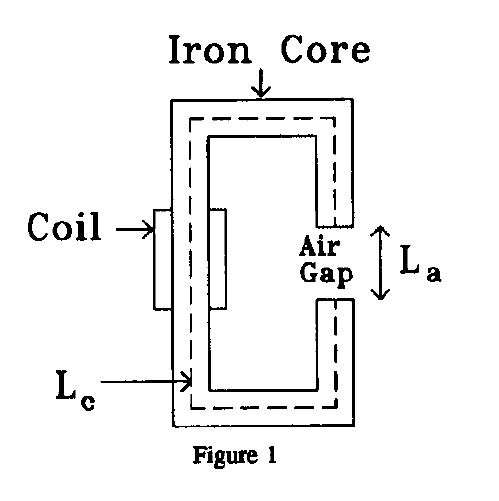
\includegraphics[width=0.8\linewidth]{mag_circuit}
				\caption{The Magnetic Circuit Discussed About}
				\label{mag_circuit}
			\end{figure}
		
			The Magnetomotive force (MMF) can be calculated by Equation \ref{mmf},
			\begin{equation}
				M = (R_g + R_c)\psi
				\label{mmf}
			\end{equation}
			where $R_g$ and $R_c$ are the reluctance of the air gap and the coil, respectively. Plug in the variables from the problem, we can transform Equation \ref{mmf} to the equation as follows:
			\begin{align*}
				M &= (\frac{l_g}{\mu_0A} + \frac{l_c}{\mu A})\psi \\
				NI &= (\frac{l_g}{\mu_0 A} + \frac{l_cH(\psi)}{AB})\psi \\
				NI &= (\frac{l_g}{\mu_0 A} + \frac{l_cH(\psi)}{\psi})\psi
			\end{align*}
			
			Simplify the equation by bringing $NI$ to the right of the equation, and the equation will be the final formula of $f(\psi)$, as is shown in Equation
			\begin{equation}
				f(\psi) = \frac{l_g \psi}{\mu_0 A} + l_cH(\psi) - NI = 0
			\end{equation}
			
			Plug in the numbers, we can finalize the equation by calculating all the coefficients of the polynomial, shown in Equation \ref{final_mmf}.
			\begin{equation}
				f(\psi) = 3.979\times 10^{7}\psi + 0.3H(\psi) - 8000
				\label{final_mmf}
			\end{equation}
			
		\subsection{Newton Raphson Method}
			This part of the problem implements the algorithm of Newton Raphson to solve the non-linear equation. The equation is shown in the previous section in Equation \ref{final_mmf}. 
			
			In the equation, there are two factors affecting the result of $f(\psi)$. One is the flux $\psi$, and the other one is the magnitude of the magnetic field $H(\psi)$. To find the magnetic field, construct a piece-wise linear interpolation shown in Figure \ref{piecewise_poly}.
			\begin{figure}[!h]
				\centering
				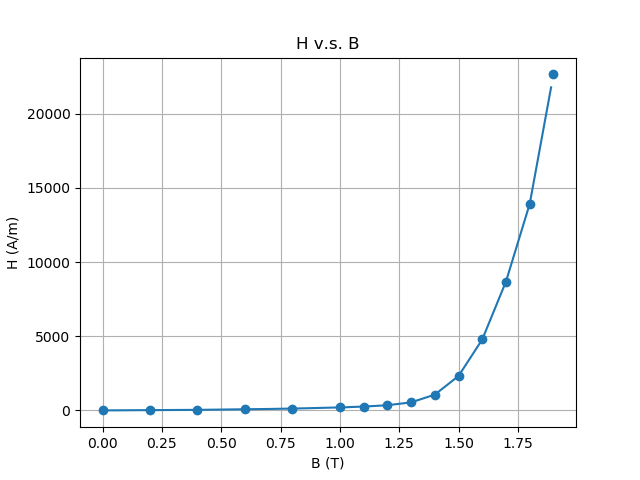
\includegraphics[width=\linewidth]{../data/Piecewise_Polynomial}
				\caption{Plot of the Piecewise Polynomial}
				\label{piecewise_poly}
			\end{figure}
		
			Note that the figure is plotted with respect to $H$ vs. $B$. and $B$ is calculated as follows:
			\begin{equation}
				B = \frac{\psi}{A}
			\end{equation}
			where A denotes the cross-sectional area. In this case, the area is $1\times 10^{-4} m^2$.
			
			Using this plot, the magnetic field magnitude can be found and $f(\psi)$ can be calculated.
			
			Listing \ref{lst:nonlinear} shows the implementation of the Newton-Raphson method. Run the main script of the assignment, Newton-Raphson returns with four iterations and a final flux of $\psi = 1.613 \times 10^{-4} Wb$, shown in Figure \ref{nr_em_result}. 
			\begin{figure}[!h]
				\centering
				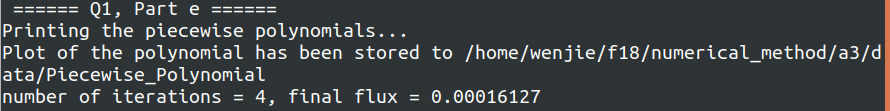
\includegraphics[width=\linewidth]{newton_raphson_em_result}
				\caption{Result of Newton-Raphson Run}
				\label{nr_em_result}
			\end{figure}
		\subsection{Successive Substitution}
			Listing \ref{lst:nonlinear} shows the implementation of successive substitution as well. The successive substitution turns out to be that the method is diverging to infinity. The reason is that the step has been too large. Therefore, I have reduced the step with a factor of $5 \times 10^{-9}$. Therefore, the method will run with smaller steps and does not miss the target point. 
			
			After the modification, the method returns with an iteration step of 483 and a flux of $1.161 \times 10^{-4} Wb$, which is similar to the result returned by Newton-Raphson, but with a much larger number of iterations, shown in Figure \ref{ss_em_result}.
			\begin{figure}[!h]
				\centering
				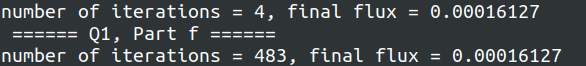
\includegraphics[width=\linewidth]{ss_em_result}
				\caption{Result of Successive Substitution Run}
				\label{ss_em_result}
			\end{figure}
	\section{The Problem of the Diode Circuit}
		\subsection{Derivation of Circuit Equation}
			
			\begin{figure}[!h]
				\centering
				\begin{circuitikz}[american voltages]
					\draw
					(0, 4) to [V, l=$E$, *-*] (0, 0)
					(0, 4) to [R, l=$R$, *-*] (4, 4) node[label={[font=\footnotesize]above:$V_1$}]{}
					to [*-*] (4, 3)
					to [diode, l=$A$, *-*] (4, 2)
					node[label={[font=\footnotesize]right:$V_2$}]{}
					to [diode, l=$B$, *-*] (4, 1)
					to [*-*] (4, 0)
					to (0, 0)
					node[ground]{}
					;
				\end{circuitikz}
				\caption{The Diode Circuit to be Investigated}
				\label{tc5}
			\end{figure}
			Figure \ref{tc5} shows the diode circuit to be investigated in this problem. Define the current flowing in the circuit to be $I$, and the current is expressed with:
			\begin{equation}
				I = \frac{E - V_1}{R}
				\label{c1}
			\end{equation}
			
			In the circuit, the current flowing through the two diodes are identical to the current flowing through the resistor. Therefore, using the diode characteristic current, the following relations can be derived:
			\begin{equation}
				I = I_{s, A}(e^{q(V_1 - V_2)/(kT)} - 1)
				\label{c2}
			\end{equation}
			and 
			\begin{equation}
				I = I_{s, B}(e^{qV_2/(kT)} - 1)
				\label{c3}
			\end{equation}
			
			From the above equations, we can derive the following two entries for the \textbf{\textit{f}} matrix, represented explicitly in terms of the variables:			
			\begin{align*}
				f_1 &= (\ref{c1}) - (\ref{c2})\\
					&= \frac{E - V_1}{R} - I_{s, A}(e^{q(V_1 - V_2)/(kT)} - 1)
			\end{align*}
			\begin{align*}
				f_2 &= (\ref{c2}) - (\ref{c3}) \\
					&= I_{s, A}(e^{q(V_1 - V_2)/(kT)} - 1) - I_{s, B}(e^{qV_2/(kT)} - 1)
			\end{align*}
			
			The \textbf{\textit{f}} matrix is then expressed as follows:
			$$
				\vec{f} = \begin{bmatrix}
					f_1 \\ f_2
				\end{bmatrix} = \begin{bmatrix}
				 0 \\ 0
				\end{bmatrix}
			$$
			
		\subsection{Solution using Newton-Raphson}
			Since this equation has output a multi-variable vector, the first step will be finding the Jacobian matrix \textbf{\textit{F}} and the multi-variable Newton Raphson update formula will be changed to:
			$$
				\textbf{\textit{V}}_n^{(k + 1)} = \textbf{\textit{V}}_n^{(k)} - \textbf{\textit{F}}^{-1(k)}\textbf{\textit{f}}^{(k)}
			$$
			
			The Jacobian matrix will be calculated following Equation as follows:
			\begin{equation}
				\textbf{\textit{F}} = \begin{bmatrix}
					\frac{\partial f_1}{\partial V_1} & \frac{\partial f_1}{\partial V_2} \\
					\frac{\partial f_2}{\partial V_1} & \frac{\partial f_2}{\partial V_2}
				\end{bmatrix}
			\end{equation}
			
			From the previous calculations for $f_1$ and $f_2$, we can derive the following expression for the four entries in the \textbf{\textit{F}} matrix:
			$$
				\frac{\partial f_1}{\partial V_1} = -\frac{1}{R} - I_{s, A}\frac{q}{kT}exp(\frac{q(V_1 - V_2)}{kT})
			$$
			$$
				\frac{\partial f_1}{\partial V_2} = I_{s,A}\frac{q}{kT}exp(\frac{q(V_1 - V_2)}{kT})
			$$
			$$
				\frac{\partial f_2}{\partial V_1} = I_{s,A}\frac{q}{kT}exp[\frac{q(V_1 - V_2)}{kT}]
			$$
			$$
				\frac{\partial f_2}{\partial V_2} = -I_{s, A}\frac{q}{kT}exp[\frac{q(V_1 - V_2)}{kT}] - I_{s, B}\frac{q}{kT}exp(\frac{qV_2}{kT})
			$$
			
			As the Jacobian matrix is a 2-by-2 matrix, its inverse can be easily calculated by:
			\begin{equation}
				\textbf{\textit{F}}^{-1} = det(\textbf{\textit{F}})\begin{bmatrix}
					d & -b \\
					-c & a
				\end{bmatrix}
			\end{equation}
			where $det(\textbf{\textit{F}})$ is calculated by:
			$$
				det(\textbf{\textit{F}}) = \frac{1}{ad - bc}
			$$
			
			The code in the main script shows the implementation of the Newton Raphson update. The error measurement is selected to be $\varepsilon_k = 1\times 10^{-6}$, and the program three iterations to converge. By running the main script, the detailed information during the iterations are shown in Figure \ref{diode_nr}.
			\begin{figure}[!h]
				\centering
				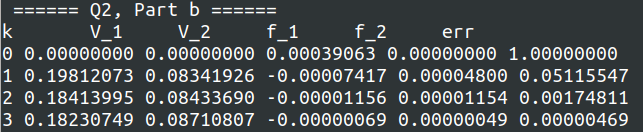
\includegraphics[width=\linewidth]{diode_nr}
				\caption{Values During Netwon Raphson Iterations}
				\label{diode_nr}
			\end{figure}
		
			To inspect if the convergence is quadratic, make a plot of the four error points shown in Figure \ref{err_measure}.
			\begin{figure}[!h]
				\centering
				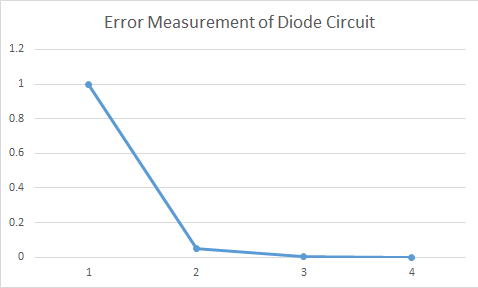
\includegraphics[width=\linewidth]{../data/diode_err}
				\caption{Plot of Error Measurement}
				\label{err_measure}
			\end{figure}
		
			From the plot, we can show the convergence to be quadratic. 
			
	\section{Gauss-Legendre Integration}
		
		
	\newpage
	\onecolumn
	\begin{appendices}
		
		\section{Code Listings} \label{appendix:code}
		
		\setminted{linenos,breaklines,fontsize=\footnotesize}
		
		\begin{center}
			\captionof{listing}{Polynomials Implementation (\texttt{polynomial.py}).}
			\inputminted{python}{../polynomial.py}
			\label{lst:poly}
		\end{center}
		\begin{center}
			\captionof{listing}{Lagrange Interpolation Implementation (\texttt{interpolation.py}).}
			\inputminted{python}{../interpolation.py}
			\label{lst:interp}
		\end{center}
		\begin{center}
			\captionof{listing}{Newton Raphson (\texttt{nonlinear.py}).}
			\inputminted{python}{../nonlinear.py}
			\label{lst:nonlinear}
		\end{center}
	\end{appendices}
\end{document}